\documentclass[crop,tikz]{standalone}
\usepackage{makeidx,fancybox,tikz,nicematrix}
\usetikzlibrary{automata, graphs,positioning, arrows,patterns,shapes.geometric,shapes.multipart,shapes.symbols,shapes.arrows}
\usetikzlibrary{arrows.meta}

%\usegdlibrary{trees,layered}
\pgfdeclarelayer{background}
\pgfdeclarelayer{foreground}
\pgfsetlayers{background,main,foreground}

\usetikzlibrary{fit, calc}
\usepackage{xparse}
\makeatletter
\NewDocumentCommand {\getnodedimen} {O{\nodewidth} O{\nodeheight} m} {
  \begin{pgfinterruptboundingbox}
  \begin{scope}[local bounding box=bb@temp]
    \node[inner sep=0pt, fit=(#3)] {};
  \end{scope}
  \path ($(bb@temp.north east)-(bb@temp.south west)$);
  \end{pgfinterruptboundingbox}
  \pgfgetlastxy{#1}{#2}
}
\makeatother

\begin{document}
 
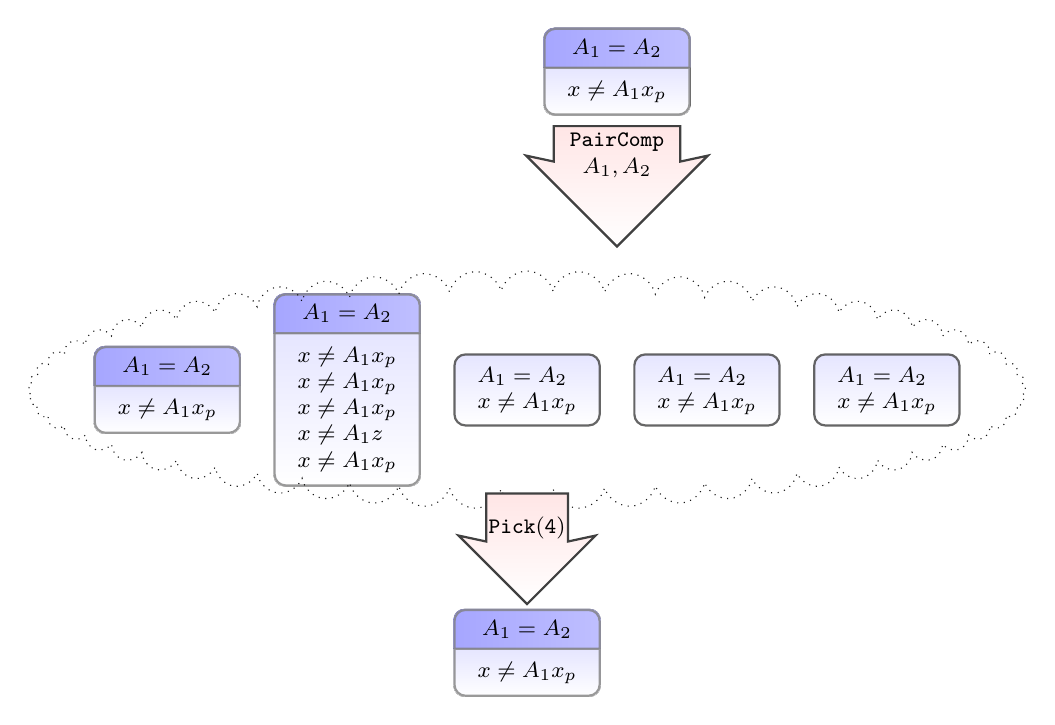
\begin{tikzpicture}
[
    level 1/.style = {sibling distance = 6.5em,level distance = 3em},
    level 2/.style = {sibling distance = 6.5em,level distance = 8.5em},
    level 3/.style = {sibling distance = 6.5em,level distance = 5em},
    level 4/.style = {sibling distance = 6.5em,level distance = 4.5em},
]

\tikzstyle{equation}=[rectangle, draw opacity=0.8,rounded corners,thick,draw=black!75,top color=blue!10, bottom color=white,minimum size=5mm, font =\footnotesize]
\tikzstyle{eqset}=[draw,cloud,inner sep=-3em,cloud puffs=60,dotted,opacity=0.9]
\tikzstyle{fullequation}=[rectangle split,rectangle split parts=2,
    rounded corners,
    thick,
    draw=black!50,
    draw opacity=0.8,
    minimum size=5mm, font =\footnotesize
    ,append after command={\pgfextra
        \fill[left color=blue!35, right color=blue!25]
    (\tikzlastnode.one west) 
    [rounded corners] |- (\tikzlastnode.north) -| (\tikzlastnode.one east) 
    [sharp corners]   |- (\tikzlastnode.one split) -| cycle;
        \fill[top color=blue!10, bottom color=white]
    (\tikzlastnode.two west) 
    [rounded corners] |- (\tikzlastnode.south) -| (\tikzlastnode.two east)  
    [sharp corners]   |- (\tikzlastnode.one split) -| cycle;
                                    \endpgfextra}]
\tikzstyle{action}=[single arrow,shape border rotate=270,inner sep=0.1ex,thick,draw=black!75,top color=red!10, bottom color=white,minimum height=4em,single arrow head extend=1em,single arrow head indent=0.5ex, font =\footnotesize,,opacity=1]
\tikzstyle{subst}=[shape aspect=4,diamond, thick,draw=black!75, top color=green!5, bottom color=white,minimum size=5mm] 
\node [fullequation]{\nodepart{one}$A_1 = A_2$\nodepart{two}$\begin{array}{l} x\neq A_1 x_{p}\end{array}$}
    child {node [action](comp1){$\begin{array}{c}\mathtt{PairComp}\\A_1,A_2\end{array}$}edge from parent [draw opacity = 0]
    child {node (c1) [fullequation]{\nodepart{one}$A_1 = A_2$\nodepart{two}$\begin{array}{l}x\neq A_1 x_{p}\end{array}$}edge from parent [draw opacity = 0]}
    child {node (c2) [fullequation]{\nodepart{one}$A_1 = A_2$\nodepart{two}$\begin{array}{l} x\neq A_1 x_{p}\\ x\neq A_1 x_{p}\\ x\neq A_1 x_{p}\\ x\neq A_1 z\\ x\neq A_1 x_{p}\end{array}$}edge from parent [draw opacity = 0]}
    child {node (c3) [equation]{$\begin{array}{l} A_1 = A_2 \\ x\neq A_1 x_{p}\end{array}$}edge from parent [draw opacity = 0]}
    child {node (c4) [equation]{$\begin{array}{l} A_1 = A_2 \\ x\neq A_1 x_{p}\end{array}$}edge from parent [draw opacity = 0]}
    child {node (c5) [equation]{$\begin{array}{l} A_1 = A_2 \\ x\neq A_1 x_{p}\end{array}$}edge from parent [draw opacity = 0]}
    child {node[eqset,aspect=5,fit=(c1) (c2) (c3) (c4) (c5)] (block1) {} 
    child {node (p1) [action] {$\mathtt{Pick(4)}$}edge from parent [draw opacity = 0]
    child {node [fullequation]{\nodepart{one}$A_1 = A_2$\nodepart{two}$\begin{array}{l} x\neq A_1 x_{p}\end{array}$}
    };
};
    };
     };
%\draw [-Stealth, thick,dashed,rounded corners] (comp1) -- (block1);
%\draw [-Stealth, thick,dashed] (c4) -- (p1);
\end{tikzpicture}

\end{document}